% Font options: 10pm, 11pt, 12pt
% Align headings left instead of center: nocenter
\documentclass[xcolor=x11names,compress]{beamer}\usepackage[]{graphicx}\usepackage[]{color}
%% maxwidth is the original width if it is less than linewidth
%% otherwise use linewidth (to make sure the graphics do not exceed the margin)
\makeatletter
\def\maxwidth{ %
  \ifdim\Gin@nat@width>\linewidth
    \linewidth
  \else
    \Gin@nat@width
  \fi
}
\makeatother

\definecolor{fgcolor}{rgb}{0.345, 0.345, 0.345}
\newcommand{\hlnum}[1]{\textcolor[rgb]{0.686,0.059,0.569}{#1}}%
\newcommand{\hlstr}[1]{\textcolor[rgb]{0.192,0.494,0.8}{#1}}%
\newcommand{\hlcom}[1]{\textcolor[rgb]{0.678,0.584,0.686}{\textit{#1}}}%
\newcommand{\hlopt}[1]{\textcolor[rgb]{0,0,0}{#1}}%
\newcommand{\hlstd}[1]{\textcolor[rgb]{0.345,0.345,0.345}{#1}}%
\newcommand{\hlkwa}[1]{\textcolor[rgb]{0.161,0.373,0.58}{\textbf{#1}}}%
\newcommand{\hlkwb}[1]{\textcolor[rgb]{0.69,0.353,0.396}{#1}}%
\newcommand{\hlkwc}[1]{\textcolor[rgb]{0.333,0.667,0.333}{#1}}%
\newcommand{\hlkwd}[1]{\textcolor[rgb]{0.737,0.353,0.396}{\textbf{#1}}}%
\let\hlipl\hlkwb

\usepackage{framed}
\makeatletter
\newenvironment{kframe}{%
 \def\at@end@of@kframe{}%
 \ifinner\ifhmode%
  \def\at@end@of@kframe{\end{minipage}}%
  \begin{minipage}{\columnwidth}%
 \fi\fi%
 \def\FrameCommand##1{\hskip\@totalleftmargin \hskip-\fboxsep
 \colorbox{shadecolor}{##1}\hskip-\fboxsep
     % There is no \\@totalrightmargin, so:
     \hskip-\linewidth \hskip-\@totalleftmargin \hskip\columnwidth}%
 \MakeFramed {\advance\hsize-\width
   \@totalleftmargin\z@ \linewidth\hsize
   \@setminipage}}%
 {\par\unskip\endMakeFramed%
 \at@end@of@kframe}
\makeatother

\definecolor{shadecolor}{rgb}{.97, .97, .97}
\definecolor{messagecolor}{rgb}{0, 0, 0}
\definecolor{warningcolor}{rgb}{1, 0, 1}
\definecolor{errorcolor}{rgb}{1, 0, 0}
\newenvironment{knitrout}{}{} % an empty environment to be redefined in TeX

\usepackage{alltt}
%\documentclass[xcolor=x11names,compress,handout]{beamer}
\usepackage[]{graphicx}
\usepackage[]{color}
\usepackage{booktabs}
\usepackage{hyperref}
\usepackage{tikz}
\usepackage{multirow}
\usepackage{multicol}
\usepackage{dcolumn}
\usepackage{bigstrut}
\usepackage{amsmath} 
\usepackage{xcolor,colortbl}
\usepackage{amssymb}
%\newcommand{\done}{\cellcolor{teal}#1}

%% Beamer Layout %%%%%%%%%%%%%%%%%%%%%%%%%%%%%%%%%%
\useoutertheme[subsection=false,shadow]{miniframes}
\useinnertheme{default}
\usefonttheme{serif}
\usepackage{Arev}
\usepackage{pdfpages}

\setbeamerfont{title like}{shape=\scshape}
\setbeamerfont{frametitle}{shape=\scshape, size=\normalsize}

\definecolor{dkblue}{RGB}{0,0,102}

\setbeamercolor*{lower separation line head}{bg=dkblue} 
\setbeamercolor*{normal text}{fg=black,bg=white} 
\setbeamercolor*{alerted text}{fg=red} 
\setbeamercolor*{example text}{fg=black} 
\setbeamercolor*{structure}{fg=black} 
 
\setbeamercolor*{palette tertiary}{fg=black,bg=black!10} 
\setbeamercolor*{palette quaternary}{fg=black,bg=black!10} 

\renewcommand{\(}{\begin{columns}}
\renewcommand{\)}{\end{columns}}
\newcommand{\<}[1]{\begin{column}{#1}}
\renewcommand{\>}{\end{column}}

\setbeamertemplate{navigation symbols}{} 
\setbeamertemplate{footline}[frame number]
\setbeamertemplate{caption}{\raggedright\insertcaption\par}

\setbeamersize{text margin left=5pt,text margin right=5pt}

%%%%%%%%%%%%%%%%%%%%%%%%%%%%%%%%%%%%%%%%%%%%%%%%%%




\title{FLS 6441 - Methods III: Explanation and Causation}
\subtitle{Week 1 - Review}
\author{Jonathan Phillips}
\date{February 2019}
\IfFileExists{upquote.sty}{\usepackage{upquote}}{}
\begin{document}

\frame{\titlepage}

\section{Introduction}

\begin{frame}
\frametitle{Course Objectives}
\begin{enumerate}
\item temp
\end{enumerate}
\end{frame}

\section{Probability}

\begin{frame}
\frametitle{Data}
\begin{enumerate}
\item We work with variables, which VARY!
\end{enumerate}
\begin{multicols}{2}
% latex table generated in R 3.5.2 by xtable 1.8-3 package
% Sat Mar 02 10:50:44 2019
\begin{table}[ht]
\centering
\begin{tabular}{rr}
  \hline
 & Variable \\ 
  \hline
1 & 0.39 \\ 
  2 & 1.69 \\ 
  3 & -1.05 \\ 
  4 & -1.38 \\ 
  5 & 0.81 \\ 
  6 & 2.01 \\ 
  7 & 0.06 \\ 
  8 & 0.98 \\ 
  9 & -0.98 \\ 
  10 & -0.39 \\ 
   \hline
\end{tabular}
\end{table}

\columnbreak
\begin{knitrout}
\definecolor{shadecolor}{rgb}{0.969, 0.969, 0.969}\color{fgcolor}
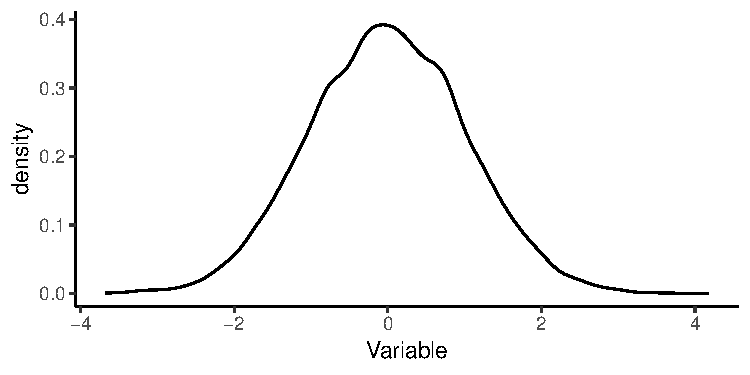
\includegraphics[width=\maxwidth]{figure/var2-1} 

\end{knitrout}
\end{multicols}
\end{frame}

% Bayes Rule: P(AnB)=P(A|B)*P(B)
% Independence: P(AnB)=P(A)*P(B) -> AIndepB. P(A|B)=P(A)
% E(x)=for random variable; (weighted) average is for sample. Same in large N/many repeated. Lecture 2, slide 69

\section{What does Regression do?}




\begin{frame}
\frametitle{Regression}
\begin{itemize}
\item Regression identifies the line through the data that minimizes the sum of squared vertical distances 
\pause
\item $y_i = \alpha + \beta D_i + \epsilon_i$
\pause
\end{itemize}
\begin{multicols}{2}
Slope = 0
\begin{knitrout}
\definecolor{shadecolor}{rgb}{0.969, 0.969, 0.969}\color{fgcolor}
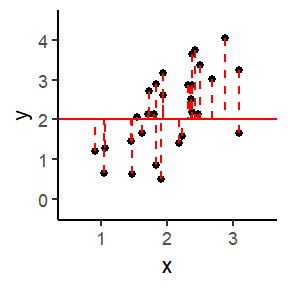
\includegraphics[width=\maxwidth]{figure/graph_ols1-1} 

\end{knitrout}
\columnbreak
Sum of Squared Residuals = 29.6
\begin{knitrout}
\definecolor{shadecolor}{rgb}{0.969, 0.969, 0.969}\color{fgcolor}
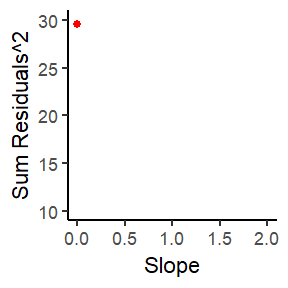
\includegraphics[width=\maxwidth]{figure/graph_ssr1-1} 

\end{knitrout}
\end{multicols}
\end{frame}

\begin{frame}
\frametitle{Regression}
\begin{itemize}
\item Regression identifies the line through the data that minimizes the sum of squared vertical distances 
\item $y_i = \alpha + \beta D_i + \epsilon_i$
\end{itemize}
\begin{multicols}{2}
Slope = 0.5
\begin{knitrout}
\definecolor{shadecolor}{rgb}{0.969, 0.969, 0.969}\color{fgcolor}
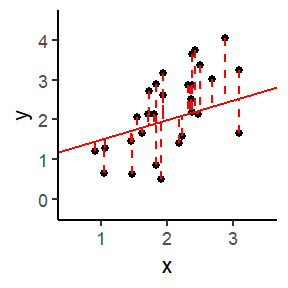
\includegraphics[width=\maxwidth]{figure/graph_ols2-1} 

\end{knitrout}
\columnbreak
Sum of Squared Residuals = 21.6
\begin{knitrout}
\definecolor{shadecolor}{rgb}{0.969, 0.969, 0.969}\color{fgcolor}
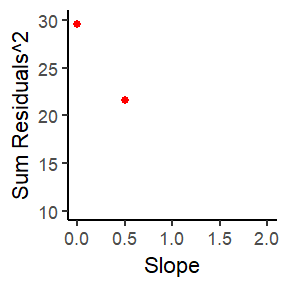
\includegraphics[width=\maxwidth]{figure/graph_ssr2-1} 

\end{knitrout}
\end{multicols}
\end{frame}

\begin{frame}
\frametitle{Regression}
\begin{itemize}
\item Regression identifies the line through the data that minimizes the sum of squared vertical distances 
\item $y_i = \alpha + \beta D_i + \epsilon_i$
\end{itemize}
\begin{multicols}{2}
Slope = 1
\begin{knitrout}
\definecolor{shadecolor}{rgb}{0.969, 0.969, 0.969}\color{fgcolor}
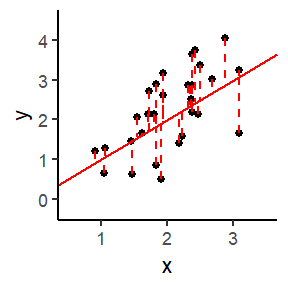
\includegraphics[width=\maxwidth]{figure/graph_ols3-1} 

\end{knitrout}
\columnbreak
Sum of Squared Residuals = 18.3
\begin{knitrout}
\definecolor{shadecolor}{rgb}{0.969, 0.969, 0.969}\color{fgcolor}
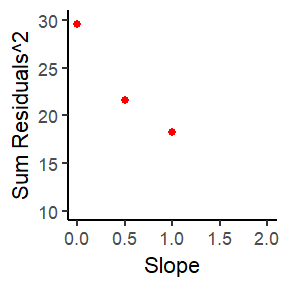
\includegraphics[width=\maxwidth]{figure/graph_ssr3-1} 

\end{knitrout}
\end{multicols}
\end{frame}

\begin{frame}
\frametitle{Regression}
\begin{itemize}
\item Regression identifies the line through the data that minimizes the sum of squared vertical distances 
\item $y_i = \alpha + \beta D_i + \epsilon_i$
\end{itemize}
\begin{multicols}{2}
Slope = 1.5
\begin{knitrout}
\definecolor{shadecolor}{rgb}{0.969, 0.969, 0.969}\color{fgcolor}
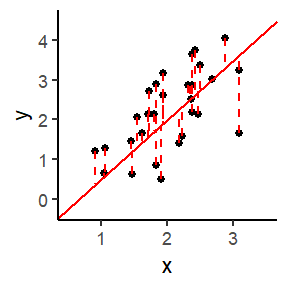
\includegraphics[width=\maxwidth]{figure/graph_ols4-1} 

\end{knitrout}
\columnbreak
Sum of Squared Residuals = 19.6
\begin{knitrout}
\definecolor{shadecolor}{rgb}{0.969, 0.969, 0.969}\color{fgcolor}
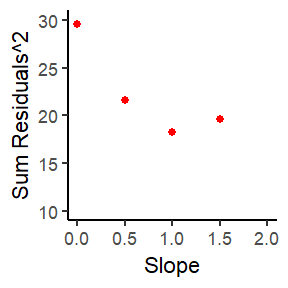
\includegraphics[width=\maxwidth]{figure/graph_ssr4-1} 

\end{knitrout}
\end{multicols}
\end{frame}

\begin{frame}
\frametitle{Regression}
\begin{itemize}
\item Regression identifies the line through the data that minimizes the sum of squared vertical distances 
\item $y_i = \alpha + \beta D_i + \epsilon_i$
\end{itemize}
\begin{multicols}{2}
Slope = 2
\begin{knitrout}
\definecolor{shadecolor}{rgb}{0.969, 0.969, 0.969}\color{fgcolor}
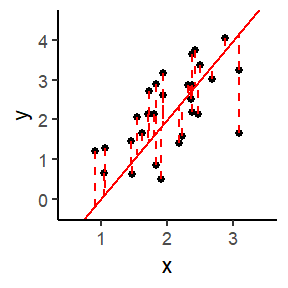
\includegraphics[width=\maxwidth]{figure/graph_ols5-1} 

\end{knitrout}
\columnbreak
Sum of Squared Residuals = 25.5
\begin{knitrout}
\definecolor{shadecolor}{rgb}{0.969, 0.969, 0.969}\color{fgcolor}
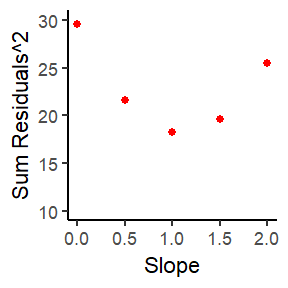
\includegraphics[width=\maxwidth]{figure/graph_ssr5-1} 

\end{knitrout}
\end{multicols}
\end{frame}

\begin{frame}
\frametitle{Regression}
\begin{itemize}
\item Regression identifies the line through the data that minimizes the sum of squared vertical distances 
\item $y_i = \alpha + \beta D_i + \epsilon_i$
\end{itemize}
\begin{multicols}{2}
Slope = 1
\begin{knitrout}
\definecolor{shadecolor}{rgb}{0.969, 0.969, 0.969}\color{fgcolor}
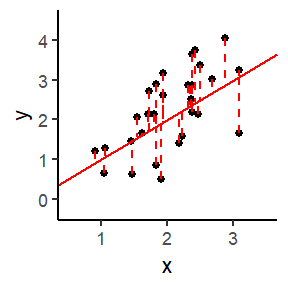
\includegraphics[width=\maxwidth]{figure/graph_ols6-1} 

\end{knitrout}
\columnbreak
Sum of Squared Residuals = 18.3
\begin{knitrout}
\definecolor{shadecolor}{rgb}{0.969, 0.969, 0.969}\color{fgcolor}
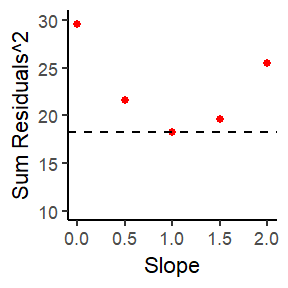
\includegraphics[width=\maxwidth]{figure/graph_ssr6-1} 

\end{knitrout}
\end{multicols}
\end{frame}

%Add noise
\begin{frame}
\frametitle{Regression}
\begin{itemize}
\item If we add pure \textit{noise} to $y$, our estimate of $\beta$ is unchanged
\begin{itemize}
\item The residual error increases
\end{itemize}
\item $y_i = \alpha + \beta D_i + \epsilon_i$
\end{itemize}
\begin{multicols}{2}
Slope = 1
\begin{knitrout}
\definecolor{shadecolor}{rgb}{0.969, 0.969, 0.969}\color{fgcolor}
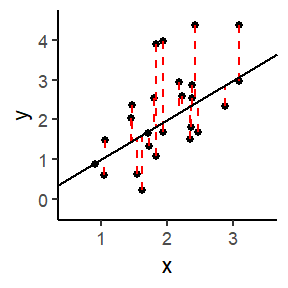
\includegraphics[width=\maxwidth]{figure/graph_ols7-1} 

\end{knitrout}
\columnbreak
Sum of Squared Residuals = 63.9
\begin{knitrout}
\definecolor{shadecolor}{rgb}{0.969, 0.969, 0.969}\color{fgcolor}
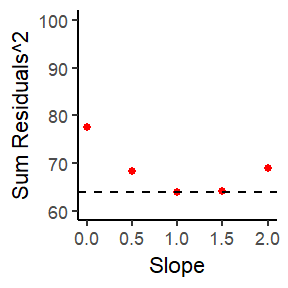
\includegraphics[width=\maxwidth]{figure/graph_ssr7-1} 

\end{knitrout}
\end{multicols}
\end{frame}

\begin{frame}
\frametitle{Regression}
\begin{itemize}
\item Dummy control variables \textit{remove variation} associated with specific levels or categories
\begin{itemize}
\item The same for fixed effects
\end{itemize}
\item $y_{ij} = \alpha + \beta D_{ij} + \tau_j + \epsilon_i$
\end{itemize}
\begin{multicols}{2}
\begin{knitrout}
\definecolor{shadecolor}{rgb}{0.969, 0.969, 0.969}\color{fgcolor}
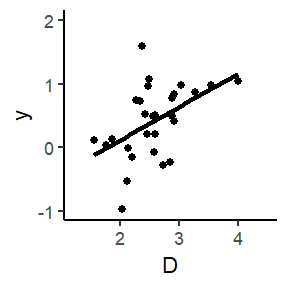
\includegraphics[width=\maxwidth]{figure/graph_ols_FE1-1} 

\end{knitrout}
\columnbreak
\end{multicols}
\end{frame}

\begin{frame}
\frametitle{Regression}
\begin{itemize}
\item Equivalently, dummy control variables restrict comparisons to within the same group:
\begin{enumerate}
\item How much does $X$ affect $Y$ within the blue group? Zero
\item How much does $X$ affect $Y$ within the red group? Zero
\item What's the average of (1) and (2) (weighted by the number of units in each group)? Zero
\end{enumerate}
\end{itemize}
\end{frame}

\begin{frame}
\frametitle{Regression}
\begin{itemize}
\item Dummy control variables \textit{remove variation} associated with specific levels or categories
\begin{itemize}
\item The same for fixed effects
\end{itemize}
\item $y_{ij} = \alpha + \beta D_{ij} + \tau_j + \epsilon_i$
\end{itemize}
\begin{multicols}{2}
\begin{knitrout}
\definecolor{shadecolor}{rgb}{0.969, 0.969, 0.969}\color{fgcolor}
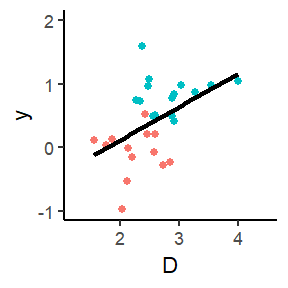
\includegraphics[width=\maxwidth]{figure/graph_ols_FE2-1} 

\end{knitrout}
\columnbreak
\end{multicols}
\end{frame}

\begin{frame}
\frametitle{Regression}
\begin{itemize}
\item Dummy control variables \textit{remove variation} associated with specific levels or categories
\begin{itemize}
\item The same for fixed effects
\end{itemize}
\item $y_{ij} = \alpha + \beta D_{ij} + \tau_j + \epsilon_i$
\end{itemize}
\begin{multicols}{2}
\begin{knitrout}
\definecolor{shadecolor}{rgb}{0.969, 0.969, 0.969}\color{fgcolor}
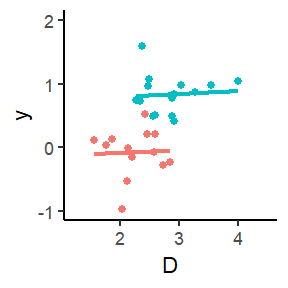
\includegraphics[width=\maxwidth]{figure/graph_ols_FE3-1} 

\end{knitrout}
\columnbreak
\end{multicols}
\end{frame}

\begin{frame}
\frametitle{Regression}
\begin{itemize}
\item Dummy control variables \textit{remove variation} associated with specific levels or categories
\begin{itemize}
\item The same for fixed effects
\end{itemize}
\item $y_{ij} = \alpha + \beta D_{ij} + \tau_j + \epsilon_i$
\end{itemize}
\begin{multicols}{2}
\begin{knitrout}
\definecolor{shadecolor}{rgb}{0.969, 0.969, 0.969}\color{fgcolor}
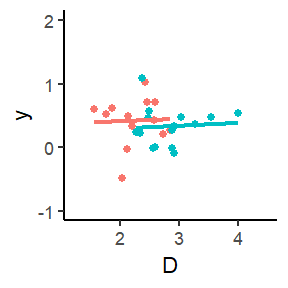
\includegraphics[width=\maxwidth]{figure/graph_ols_FE4-1} 

\end{knitrout}
\columnbreak
\end{multicols}
\end{frame}

\begin{frame}
\frametitle{Regression}
\begin{itemize}
\item Dummy control variables \textit{remove variation} associated with specific levels or categories
\begin{itemize}
\item The same for fixed effects
\end{itemize}
\item $y_{ij} = \alpha + \beta D_{ij} + \tau_j + \epsilon_i$
\end{itemize}
\begin{multicols}{2}
\begin{knitrout}
\definecolor{shadecolor}{rgb}{0.969, 0.969, 0.969}\color{fgcolor}
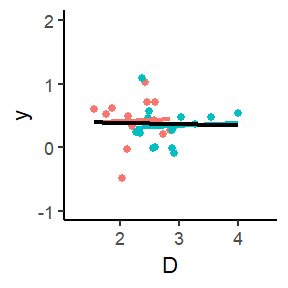
\includegraphics[width=\maxwidth]{figure/graph_ols_FE5-1} 

\end{knitrout}
\columnbreak
\end{multicols}
\end{frame}

\begin{frame}
\frametitle{Regression}
\begin{itemize}
\item Continuous control variables \textit{remove variation} based on how much the control explains $y$
\item $y_i = \alpha + \beta_1 D_i + \beta_2 X_i + \epsilon_i$
\end{itemize}
\begin{multicols}{2}
\begin{knitrout}
\definecolor{shadecolor}{rgb}{0.969, 0.969, 0.969}\color{fgcolor}
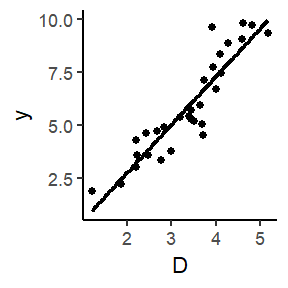
\includegraphics[width=\maxwidth]{figure/graph_ols_control1-1} 

\end{knitrout}
\columnbreak

The coefficient on $D$ is 1.503
Real coefficient = 1
\end{multicols}
\end{frame}

\begin{frame}
\frametitle{Regression}
\begin{itemize}
\item Continuous control variables \textit{remove variation} based on how much the control explains $y$
\item $y_i = \alpha + \beta_1 D_i + \beta_2 X_i + \epsilon_i$
\end{itemize}
\begin{multicols}{2}
\begin{knitrout}
\definecolor{shadecolor}{rgb}{0.969, 0.969, 0.969}\color{fgcolor}
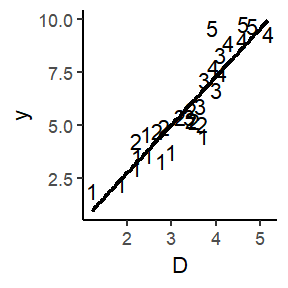
\includegraphics[width=\maxwidth]{figure/graph_ols_control2-1} 

\end{knitrout}
\columnbreak
The coefficient on $D$ is 1.503
Real coefficient = 1
\end{multicols}
\end{frame}

\begin{frame}
\frametitle{Regression}
\begin{itemize}
\item Continuous control variables \textit{remove variation} based on how much the control explains $y$
\item $y_i = \alpha + \beta_1 D_i + \beta_2 X_i + \epsilon_i$
\end{itemize}
\begin{multicols}{2}
\begin{knitrout}
\definecolor{shadecolor}{rgb}{0.969, 0.969, 0.969}\color{fgcolor}
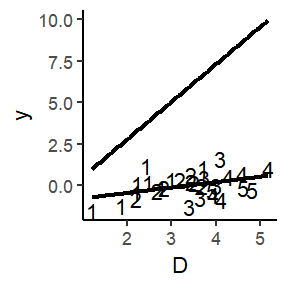
\includegraphics[width=\maxwidth]{figure/graph_ols_control3-1} 

\end{knitrout}
\columnbreak

The coefficient on $D$ is 0.991
Real coefficient = 1
\end{multicols}
\end{frame}

%Next, with no overlap for binary treatment to show role of linearity

%epsilon larger when more dispersed around line with same slope

\begin{frame}
\frametitle{Regression}
\begin{itemize}
\item Regression is a \textbf{Conditional Expectation Function}
\pause
\item Conditional on $x$, what is our expectation (mean value) of $y$?
\pause
\item $E(y|x)$
\pause
\item When age is 20 ($x=40$), the average salary is R1.000 ($y=1.000$)
\item When age is 40 ($x=40$), the average salary is R2.000 ($y=2.000$)
\end{itemize}
\end{frame}

\begin{frame}
\frametitle{Regression}
\begin{itemize}
\item Regression is a \textbf{Conditional Expectation Function}: $E(y|x)$
\pause
\item It predicts the \textbf{mean}, not the median, not the minimum, not the maximum
\end{itemize}
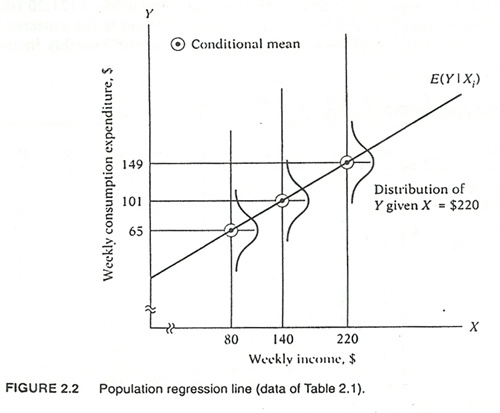
\includegraphics[width=0.75\textwidth]{CEF.jpg}
\end{frame}

\begin{frame}
\frametitle{Regression}
$$\hat{\beta_1}=\frac{\sum_i (x_i - \bar{x})(y_i - \bar{y})}{\sum_i (x_i - \bar{x})^2}$$
$$\hat{\beta_0}=\bar{y} - \hat{\beta_1} \bar{x}$$
\end{frame}



\begin{frame}
\frametitle{Regression}
\begin{itemize}
\item Regression with two variables is very similar to calculating correlation
\pause
\item $\hat{\beta}=cor(x,y) * \frac{\sigma_Y}{\sigma_X}$
\pause
\item It's \textit{identical} if we standardize both variables first ($\frac{(x-\bar{x})}{\sigma_x}$)
\pause
\end{itemize}
\begin{multicols}{2}
\begin{knitrout}
\definecolor{shadecolor}{rgb}{0.969, 0.969, 0.969}\color{fgcolor}
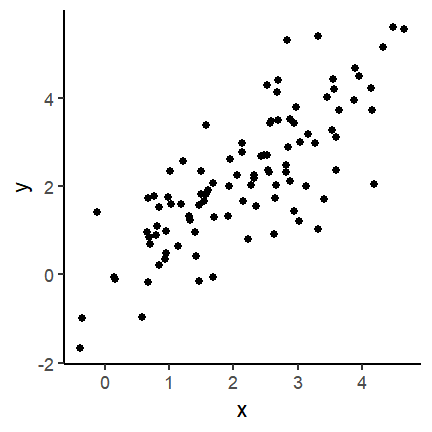
\includegraphics[width=\maxwidth]{figure/corr_regn_fig1-1} 

\end{knitrout}
\columnbreak
\end{multicols}
\end{frame}

\begin{frame}
\frametitle{Regression}
\begin{itemize}
\item Regression with two variables is very similar to calculating correlation:
\item $\hat{\beta}=cor(x,y) * \frac{\sigma_Y}{\sigma_X}$
\item It's \textit{identical} if we standardize both variables first ($\frac{(x-\bar{x})}{\sigma_x}$)
\end{itemize}
\begin{multicols}{2}
\begin{knitrout}
\definecolor{shadecolor}{rgb}{0.969, 0.969, 0.969}\color{fgcolor}
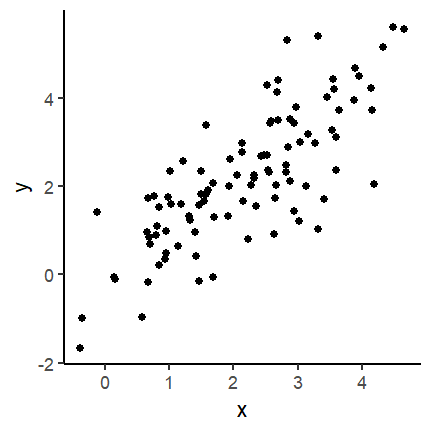
\includegraphics[width=\maxwidth]{figure/corr_regn_fig2-1} 

\end{knitrout}
\columnbreak
\begin{itemize}
\item Correlation is 0.781
\pause
\item Regression Results:
\end{itemize}
% latex table generated in R 3.5.2 by xtable 1.8-3 package
% Sat Mar 02 10:51:08 2019
\begin{table}[ht]
\centering
\begin{tabular}{rlr}
  \hline
 & term & estimate \\ 
  \hline
1 & (Intercept) & 0.006 \\ 
  2 & x & 1.008 \\ 
   \hline
\end{tabular}
\end{table}

\end{multicols}
\end{frame}

\begin{frame}
\frametitle{Regression}
\begin{itemize}
\item Regression with two variables is very similar to calculating correlation:
\item $\hat{\beta}=cor(x,y) * \frac{\sigma_Y}{\sigma_X}$
\item It's \textit{identical} if we standardize both variables first ($\frac{(x-\bar{x})}{\sigma_x}$)
\end{itemize}
\begin{multicols}{2}
\begin{knitrout}
\definecolor{shadecolor}{rgb}{0.969, 0.969, 0.969}\color{fgcolor}
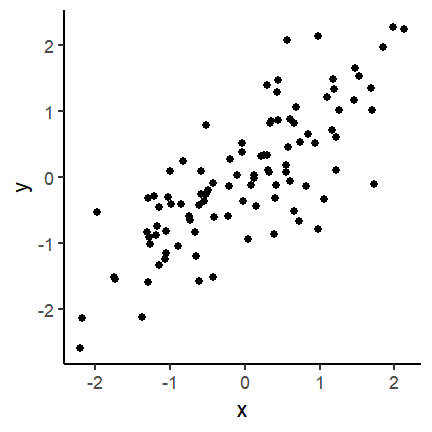
\includegraphics[width=\maxwidth]{figure/corr_regn_fig3-1} 

\end{knitrout}
\columnbreak
\begin{itemize}
\item Correlation is 0.781
\item Standardized Regression Results:
\end{itemize}
% latex table generated in R 3.5.2 by xtable 1.8-3 package
% Sat Mar 02 10:51:11 2019
\begin{table}[ht]
\centering
\begin{tabular}{rlr}
  \hline
 & term & estimate \\ 
  \hline
1 & (Intercept) & 0.000 \\ 
  2 & x & 0.781 \\ 
   \hline
\end{tabular}
\end{table}

\end{multicols}
\end{frame}

\begin{frame}
\frametitle{Regression}
\begin{itemize}
\item Regression with \textbf{multiple} variables is very similar to calculating \textbf{partial} correlation:
\pause
\item Just a small difference in the denominator (how we standardize the measure)
\pause
\end{itemize}
$$\beta_{x_1} = \frac{r_{yx_1} - r_{yx_2}r_{x_1x_2}}{1-r^2_{x_1x_2}}$$
$$r_{yx_1|x_2} = \frac{r_{yx_1} - r_{yx_2}r_{x_1x_2}}{\sqrt{(1-r^2_{yx_2})(1-r^2_{x_1x_2})}}$$
\begin{itemize}
\item \textbf{There is no magic in regression, it's just correlation 'extra'}
\end{itemize}
\end{frame}

\begin{frame}
\frametitle{Regression}
\begin{itemize}
\item We \textbf{NEVER} know the true value of $\beta$
\pause
\item We \textbf{estimate a distribution} for $\beta$
\end{itemize}
\begin{knitrout}
\definecolor{shadecolor}{rgb}{0.969, 0.969, 0.969}\color{fgcolor}
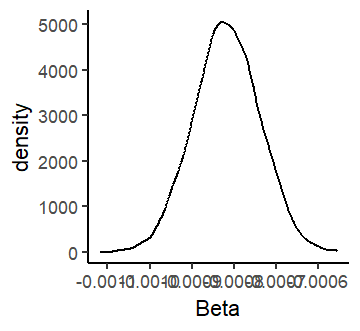
\includegraphics[width=\maxwidth]{figure/beta_dist-1} 

\end{knitrout}
\end{frame}

\begin{frame}
\frametitle{Regression}
\begin{itemize}
\item We \textbf{NEVER} know the true value of $\beta$
\item We \textbf{estimate a distribution} for $\beta$
\end{itemize}
\begin{knitrout}
\definecolor{shadecolor}{rgb}{0.969, 0.969, 0.969}\color{fgcolor}
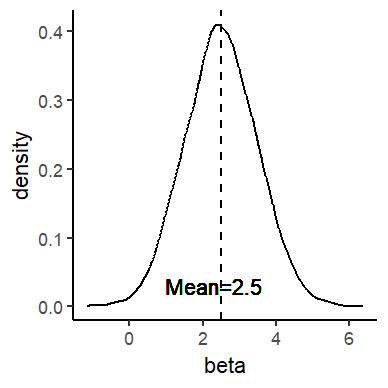
\includegraphics[width=\maxwidth]{figure/beta_dist2-1} 

\end{knitrout}
\end{frame}

\begin{frame}
\frametitle{Regression}
\begin{itemize}
\item We \textbf{NEVER} know the true value of $\beta$
\item We \textbf{estimate a distribution} for $\beta$
\end{itemize}
\begin{knitrout}
\definecolor{shadecolor}{rgb}{0.969, 0.969, 0.969}\color{fgcolor}
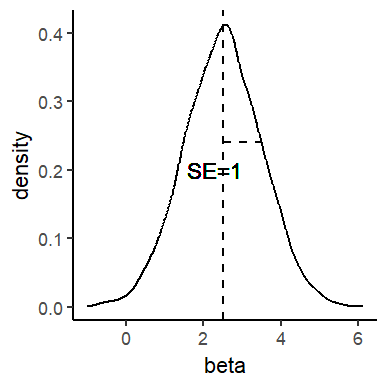
\includegraphics[width=\maxwidth]{figure/beta_dist3-1} 

\end{knitrout}
\end{frame}

\begin{frame}
\frametitle{Regression}
\begin{itemize}
\item We \textbf{NEVER} know the true value of $\beta$
\item We \textbf{estimate a distribution} for $\beta$
\end{itemize}
\begin{knitrout}
\definecolor{shadecolor}{rgb}{0.969, 0.969, 0.969}\color{fgcolor}
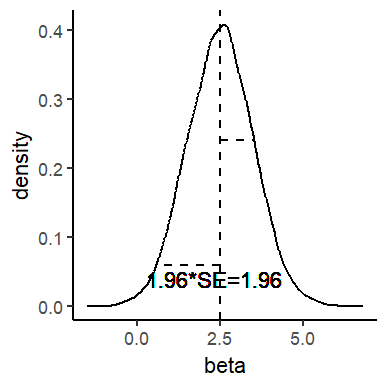
\includegraphics[width=\maxwidth]{figure/beta_dist4-1} 

\end{knitrout}
\end{frame}

\begin{frame}
\frametitle{Regression}
\begin{itemize}
\item We \textbf{NEVER} know the true value of $\beta$
\item We \textbf{estimate a distribution} for $\beta$
\end{itemize}
\begin{knitrout}
\definecolor{shadecolor}{rgb}{0.969, 0.969, 0.969}\color{fgcolor}
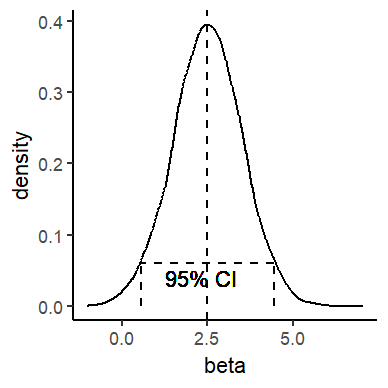
\includegraphics[width=\maxwidth]{figure/beta_dist5-1} 

\end{knitrout}
\end{frame}


\section{Guide to Designing Regressions}

\begin{frame}
\frametitle{Regression Guide}
\begin{enumerate}
\item \textbf{Choose variables and measures:} To test a specific hypothesis
\item \textbf{Choose a Model/Link Function:} Should match the data type of your outcome variable
\item \textbf{Choose Covariates:} To match your strategy of inference
\item \textbf{Choose Fixed Effects:} To focus on a specific level of variation
\item \textbf{Choose Error Structure:} To match known dependencies/clustering in the data
\item \textbf{Interpret the coefficients:} Depending on the type/scale of the explanatory variable
\end{enumerate}
\end{frame}

\begin{frame}
\frametitle{2. Regression Models}
The Regression Model reflects the data type of the outcome variable:
\begin{itemize}
\item Continuous -> Ordinary Least Squares  
\begin{knitrout}
\definecolor{shadecolor}{rgb}{0.969, 0.969, 0.969}\color{fgcolor}\begin{kframe}
\begin{alltt}
\hlkwd{zelig}\hlstd{(Y} \hlopt{~} \hlstd{X,}\hlkwc{data}\hlstd{=d,}\hlkwc{model}\hlstd{=}\hlstr{"ls"}\hlstd{)}
\end{alltt}
\end{kframe}
\end{knitrout}
\item Binary -> Logit  
\begin{knitrout}
\definecolor{shadecolor}{rgb}{0.969, 0.969, 0.969}\color{fgcolor}\begin{kframe}
\begin{alltt}
\hlkwd{zelig}\hlstd{(Y} \hlopt{~} \hlstd{X,}\hlkwc{data}\hlstd{=d,}\hlkwc{model}\hlstd{=}\hlstr{"logit"}\hlstd{)}
\end{alltt}
\end{kframe}
\end{knitrout}
\item Unordered categories -> Multinomial logit  
\begin{knitrout}
\definecolor{shadecolor}{rgb}{0.969, 0.969, 0.969}\color{fgcolor}\begin{kframe}
\begin{alltt}
\hlkwd{zelig}\hlstd{(Y} \hlopt{~} \hlstd{X,}\hlkwc{data}\hlstd{=d,}\hlkwc{model}\hlstd{=}\hlstr{"mlogit"}\hlstd{)}
\end{alltt}
\end{kframe}
\end{knitrout}
\item Ordered categories -> Ordered logit  
\begin{knitrout}
\definecolor{shadecolor}{rgb}{0.969, 0.969, 0.969}\color{fgcolor}\begin{kframe}
\begin{alltt}
\hlkwd{zelig}\hlstd{(Y} \hlopt{~} \hlstd{X,}\hlkwc{data}\hlstd{=d,}\hlkwc{model}\hlstd{=}\hlstr{"ologit"}\hlstd{)}
\end{alltt}
\end{kframe}
\end{knitrout}
\item Count -> Poisson  
\begin{knitrout}
\definecolor{shadecolor}{rgb}{0.969, 0.969, 0.969}\color{fgcolor}\begin{kframe}
\begin{alltt}
\hlkwd{zelig}\hlstd{(Y} \hlopt{~} \hlstd{X,}\hlkwc{data}\hlstd{=d,}\hlkwc{model}\hlstd{=}\hlstr{"poisson"}\hlstd{)}
\end{alltt}
\end{kframe}
\end{knitrout}
\end{itemize}
\end{frame}

\begin{frame}
\frametitle{6. Interpreting Regression Results}
\begin{itemize}
\item Difficult! It depends on the scale of the explanatory variable, scale of the outcome, the regression model we used, and the presence of any interaction
\item Basic OLS:
\begin{itemize}
\item 1 [unit of explanatory variable] change in the explanatory variable is associated with a $\beta$ [unit of outcome variable] change in the outcome
\end{itemize}
\end{itemize}
\end{frame}



\begin{frame}
\frametitle{Predictions from Regressions}
\begin{itemize}
\item The coefficient on the regression of income on attitude to redistribution is -0.000818
\begin{itemize}
\pause
\item So??? What do we learn from this?
\pause
\item Coefficients are hard to interpret, and depend on how we measure each variable
\item And p-values are arbitrary
\end{itemize}  
\pause
\item Better to make specific \textit{predictions} of how changes in $X$ produce changes in $Y$
\end{itemize}
\end{frame}

\begin{frame}
\frametitle{Predictions from Regressions}
$$Attitude_i = \alpha + \beta_1 \text{ Income}_i + \epsilon_i$$ \\
\pause
$$Attitude_i = 2.235 - 0.000818 \text{ Income}_i + N(0,2.378)$$ \\
\pause
\textbf{If Income is 3000:}  \\
$$Attitude_i = 2.235-0.000818*3000 + N(0,2.378)$$ \\
$$Attitude_i = -0.219 + N(0,2.378)$$
\end{frame}

\begin{frame}
\frametitle{Predictions from Regressions}
$$Attitude_i = \alpha + \beta_1 \text{ Income}_i + \epsilon_i$$ \\
$$Attitude_i = 2.235 - 0.000818 \text{ Income}_i + N(0,2.378)$$ \\
\textbf{If Income is 6000:}  \\
$$Attitude_i = 2.235-0.000818*6000 + N(0,2.378)$$ \\
$$Attitude_i = -2.673 + N(0,2.378)$$
\end{frame}

\begin{frame}
\frametitle{Predictions from Regressions}
$$Attitude_i = \alpha + \beta_1 \text{ Income}_i + \epsilon_i$$
$$Attitude_i = 2.235 - 0.000818 \text{ Income}i + N(0,2.378)$$
\textbf{Increasing Income from 3000 to 6000:} \\
$$\Delta Attitude_i = (2.235-0.000818*6000) - (2.235-0.000818*3000)$$
$$\Delta Attitude_i = -2.673 - -0.219$$
$$\Delta Attitude_i = -2.454$$
\end{frame}

\begin{frame}
\frametitle{Predictions from Regressions}
\begin{knitrout}
\definecolor{shadecolor}{rgb}{0.969, 0.969, 0.969}\color{fgcolor}
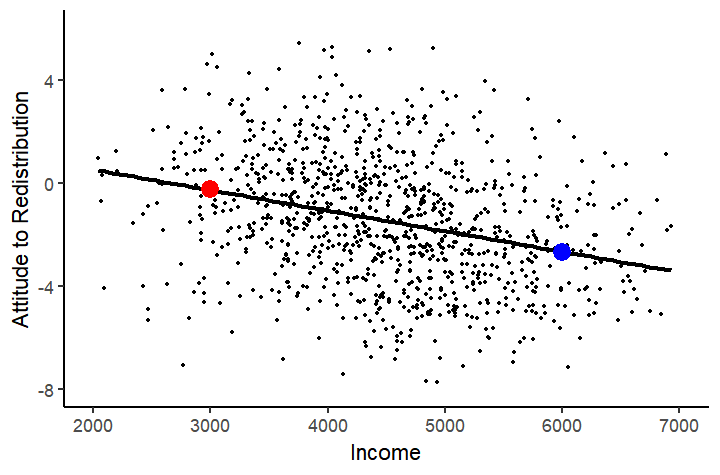
\includegraphics[width=\maxwidth]{figure/predictions1-1} 

\end{knitrout}
\end{frame}

\begin{frame}
\frametitle{Predictions from Regressions}
\begin{multicols}{2}
Predicted Values:
\begin{knitrout}
\definecolor{shadecolor}{rgb}{0.969, 0.969, 0.969}\color{fgcolor}
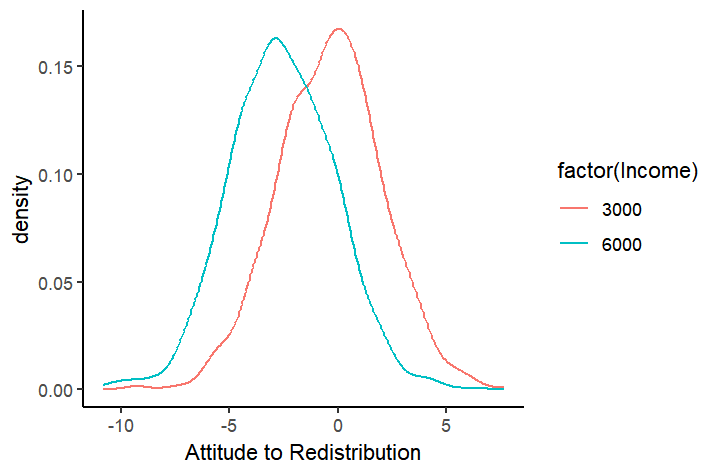
\includegraphics[width=\maxwidth]{figure/predictions2-1} 

\end{knitrout}
\columnbreak
First Differences:
\begin{knitrout}
\definecolor{shadecolor}{rgb}{0.969, 0.969, 0.969}\color{fgcolor}
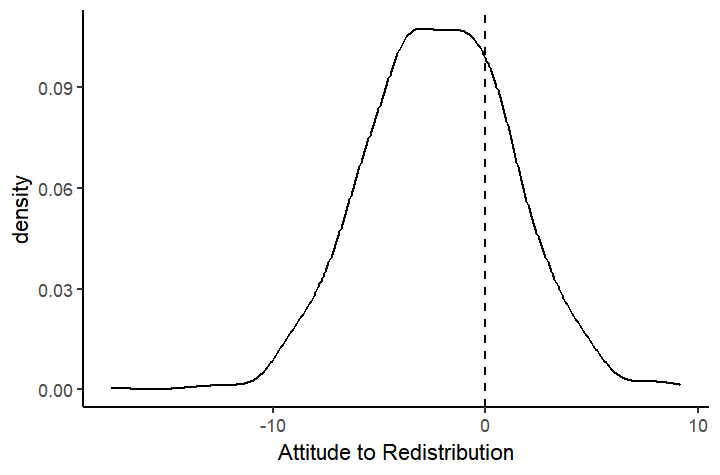
\includegraphics[width=\maxwidth]{figure/predictions3-1} 

\end{knitrout}
\end{multicols}
\end{frame}

\begin{frame}
\frametitle{Predictions from Regressions}
\begin{itemize}
\item The regression model matters because the wrong model makes non-sensical predictions
\item Consider a binary outcome: $Gender_i = \alpha + \beta Income_i + \epsilon_i$
\item Compare the OLS and Logit regression tables:
\end{itemize}
\begin{multicols}{2}

% Table created by stargazer v.5.2.2 by Marek Hlavac, Harvard University. E-mail: hlavac at fas.harvard.edu
% Date and time: Thu, Mar 07, 2019 - 8:44:04 AM
\begin{table}[!htbp] \centering 
  \caption{} 
  \label{} 
\tiny 
\begin{tabular}{@{\extracolsep{1pt}}lc} 
\\[-1.8ex]\hline 
\hline \\[-1.8ex] 
 & \multicolumn{1}{c}{\textit{Dependent variable:}} \\ 
\cline{2-2} 
\\[-1.8ex] & as.numeric(as.character(gender)) \\ 
\hline \\[-1.8ex] 
 income & 0.0003$^{***}$ (0.00001) \\ 
  Constant & $-$0.696$^{***}$ (0.066) \\ 
 \hline \\[-1.8ex] 
Observations & 1,000 \\ 
\hline 
\hline \\[-1.8ex] 
\textit{Note:}  & \multicolumn{1}{r}{$^{*}$p$<$0.1; $^{**}$p$<$0.05; $^{***}$p$<$0.01} \\ 
\end{tabular} 
\end{table} 

\columnbreak

% Table created by stargazer v.5.2.2 by Marek Hlavac, Harvard University. E-mail: hlavac at fas.harvard.edu
% Date and time: Thu, Mar 07, 2019 - 8:44:05 AM
\begin{table}[!htbp] \centering 
  \caption{} 
  \label{} 
\tiny 
\begin{tabular}{@{\extracolsep{1pt}}lc} 
\\[-1.8ex]\hline 
\hline \\[-1.8ex] 
 & \multicolumn{1}{c}{\textit{Dependent variable:}} \\ 
\cline{2-2} 
\\[-1.8ex] & as.numeric(as.character(gender)) \\ 
\hline \\[-1.8ex] 
 income & 0.001$^{***}$ (0.0001) \\ 
  Constant & $-$6.360$^{***}$ (0.457) \\ 
 \hline \\[-1.8ex] 
Observations & 1,000 \\ 
\hline 
\hline \\[-1.8ex] 
\textit{Note:}  & \multicolumn{1}{r}{$^{*}$p$<$0.1; $^{**}$p$<$0.05; $^{***}$p$<$0.01} \\ 
\end{tabular} 
\end{table} 

\end{multicols}
\end{frame}

\begin{frame}
\frametitle{Predictions from Regressions}
\begin{itemize}
\item The regression model matters because the wrong model makes non-sensical predictions
\item Consider a binary outcome: $Gender_i = \alpha + \beta Income_i + \epsilon_i$
\item Compare the OLS and Logit \textbf{predictions} of gender for an income of R\$3000:
\end{itemize}
\begin{multicols}{2}
\begin{knitrout}
\definecolor{shadecolor}{rgb}{0.969, 0.969, 0.969}\color{fgcolor}
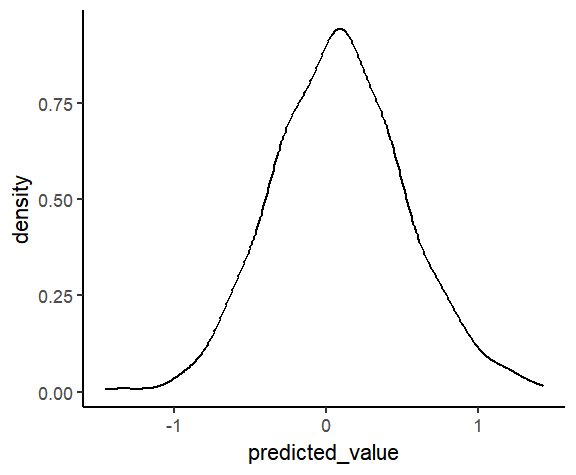
\includegraphics[width=\maxwidth]{figure/preds_1_ols_chart-1} 

\end{knitrout}
\columnbreak
\begin{knitrout}
\definecolor{shadecolor}{rgb}{0.969, 0.969, 0.969}\color{fgcolor}
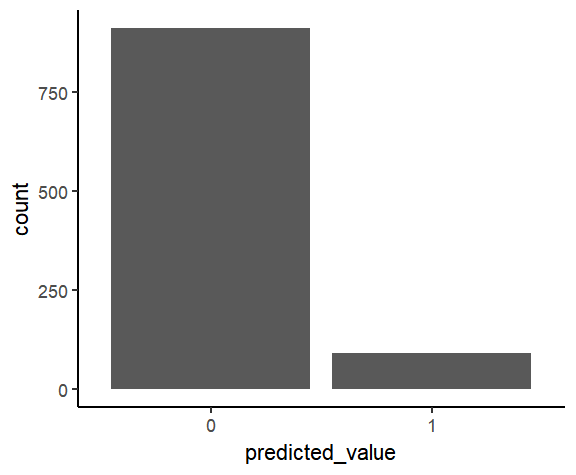
\includegraphics[width=\maxwidth]{figure/preds_1_logit_chart-1} 

\end{knitrout}
\end{multicols}
\end{frame}

\section{What does Regression NOT do?}

\begin{frame}
\frametitle{Omitted Variable Bias}
\begin{knitrout}
\definecolor{shadecolor}{rgb}{0.969, 0.969, 0.969}\color{fgcolor}
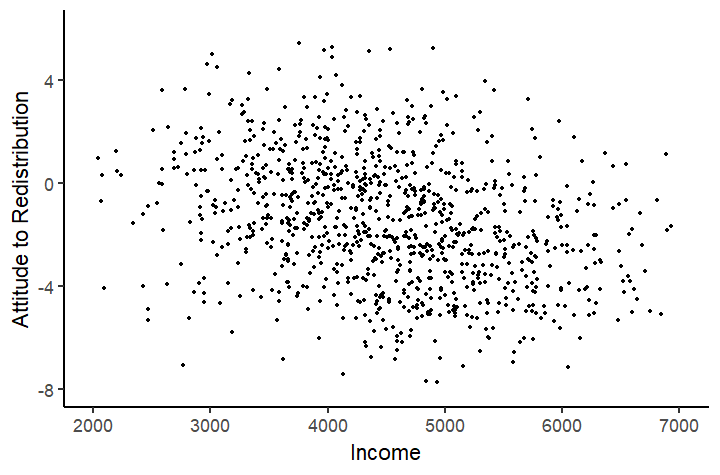
\includegraphics[width=\maxwidth]{figure/confound3b-1} 

\end{knitrout}
\end{frame}

\begin{frame}
\frametitle{Omitted Variable Bias}
\begin{knitrout}
\definecolor{shadecolor}{rgb}{0.969, 0.969, 0.969}\color{fgcolor}
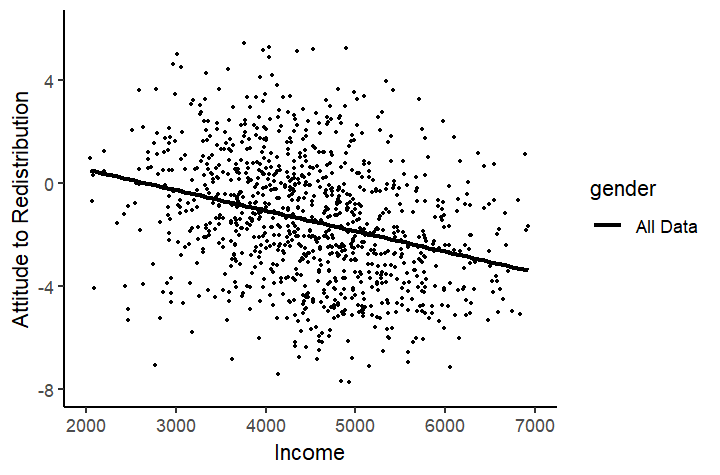
\includegraphics[width=\maxwidth]{figure/confound3c-1} 

\end{knitrout}
\end{frame}

\begin{frame}
\frametitle{Omitted Variable Bias}
\begin{knitrout}
\definecolor{shadecolor}{rgb}{0.969, 0.969, 0.969}\color{fgcolor}
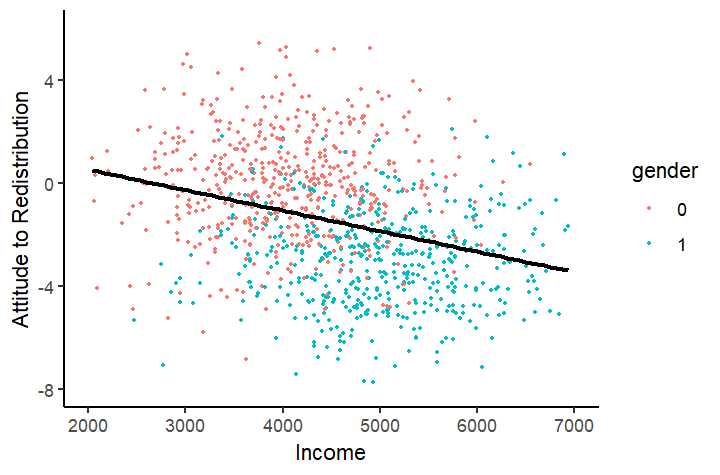
\includegraphics[width=\maxwidth]{figure/confound2-1} 

\end{knitrout}
\end{frame}


\begin{frame}
\frametitle{Omitted Variable Bias}
\begin{knitrout}
\definecolor{shadecolor}{rgb}{0.969, 0.969, 0.969}\color{fgcolor}
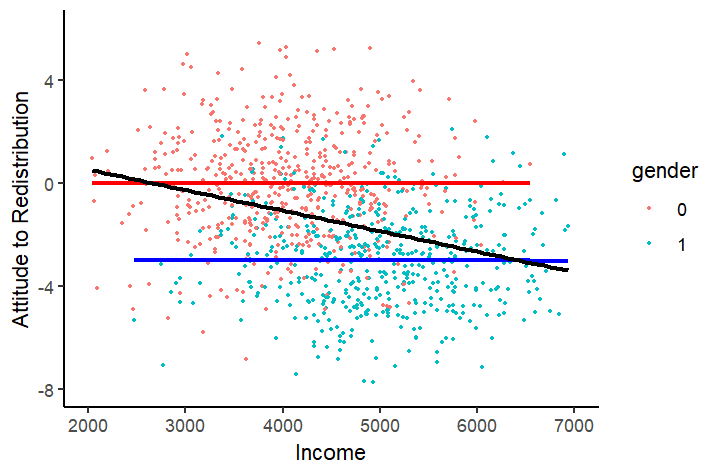
\includegraphics[width=\maxwidth]{figure/confound3-1} 

\end{knitrout}
\end{frame}

\begin{frame}
\frametitle{Reverse Causation}
\begin{itemize}
\item Significant regression coefficients just reflect the values in our dataset moving together
\pause
\item Does the 'direction' of regression  matter? I.e. Does regression treat $X$ and $Y$ differently?
\pause
\item Yes! 
\begin{multicols}{2}

% Table created by stargazer v.5.2.2 by Marek Hlavac, Harvard University. E-mail: hlavac at fas.harvard.edu
% Date and time: Wed, Mar 06, 2019 - 12:10:54 PM
\begin{table}[!htbp] \centering 
  \caption{} 
  \label{} 
\tiny 
\begin{tabular}{@{\extracolsep{1pt}}lc} 
\\[-1.8ex]\hline 
\hline \\[-1.8ex] 
 & \multicolumn{1}{c}{\textit{Dependent variable:}} \\ 
\cline{2-2} 
\\[-1.8ex] & redist \\ 
\hline \\[-1.8ex] 
 income & $-$0.011 (0.029) \\ 
  gender1 & $-$1.201$^{***}$ (0.058) \\ 
  Constant & 0.589$^{***}$ (0.038) \\ 
 \hline \\[-1.8ex] 
Observations & 1,000 \\ 
\hline 
\hline \\[-1.8ex] 
\textit{Note:}  & \multicolumn{1}{r}{$^{*}$p$<$0.1; $^{**}$p$<$0.05; $^{***}$p$<$0.01} \\ 
\end{tabular} 
\end{table} 

\columnbreak

% Table created by stargazer v.5.2.2 by Marek Hlavac, Harvard University. E-mail: hlavac at fas.harvard.edu
% Date and time: Wed, Mar 06, 2019 - 12:10:55 PM
\begin{table}[!htbp] \centering 
  \caption{} 
  \label{} 
\tiny 
\begin{tabular}{@{\extracolsep{1pt}}lc} 
\\[-1.8ex]\hline 
\hline \\[-1.8ex] 
 & \multicolumn{1}{c}{\textit{Dependent variable:}} \\ 
\cline{2-2} 
\\[-1.8ex] & income \\ 
\hline \\[-1.8ex] 
 redist & $-$0.013 (0.034) \\ 
  gender1 & 0.993$^{***}$ (0.069) \\ 
  Constant & $-$0.487$^{***}$ (0.043) \\ 
 \hline \\[-1.8ex] 
Observations & 1,000 \\ 
\hline 
\hline \\[-1.8ex] 
\textit{Note:}  & \multicolumn{1}{r}{$^{*}$p$<$0.1; $^{**}$p$<$0.05; $^{***}$p$<$0.01} \\ 
\end{tabular} 
\end{table} 

\end{multicols}
\item Remember, regression measures the \textit{vertical} (not diagonal) distances to the regression line
\begin{itemize}
\item It minimizes the prediction errors for $Y$
\end{itemize}
\item But that doesn't mean it identifies the direction of causation!
\end{itemize}
\end{frame}

\begin{frame}
\frametitle{Selection Bias}
\begin{itemize}
\item There are four selection risks:
\begin{enumerate}
\item \textbf{Selection into existence}
\item \textbf{Selection into survival}
\item \textbf{Selection into the dataset}
\item \textbf{Selection into treatment}
\end{enumerate}
\item In each case, we don't see the \textit{full} relationship between $X$ and $Y$
\item So our regression estimates are biased
\end{itemize}
\end{frame}

\begin{frame}
\frametitle{Selection Bias}
\begin{itemize}
\item Imagine we do not see 'rich' units with high income (above R\$4000)
\end{itemize}
\begin{knitrout}
\definecolor{shadecolor}{rgb}{0.969, 0.969, 0.969}\color{fgcolor}
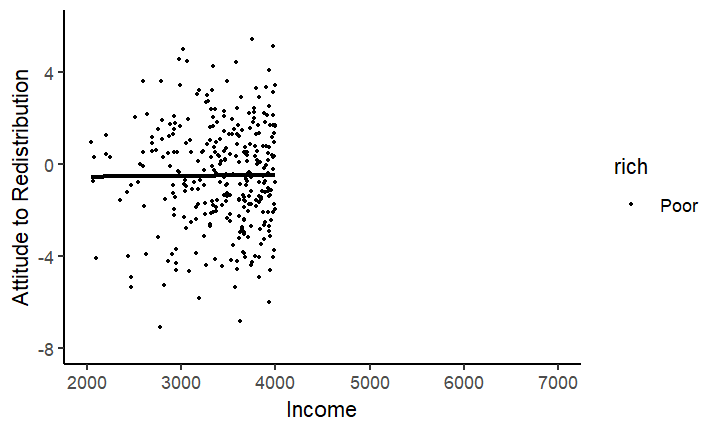
\includegraphics[width=\maxwidth]{figure/selection1-1} 

\end{knitrout}
\end{frame}

\begin{frame}
\frametitle{Selection Bias}
\begin{itemize}
\item Imagine we do not see 'rich' units with high income (above R\$4000)
\end{itemize}
\begin{knitrout}
\definecolor{shadecolor}{rgb}{0.969, 0.969, 0.969}\color{fgcolor}
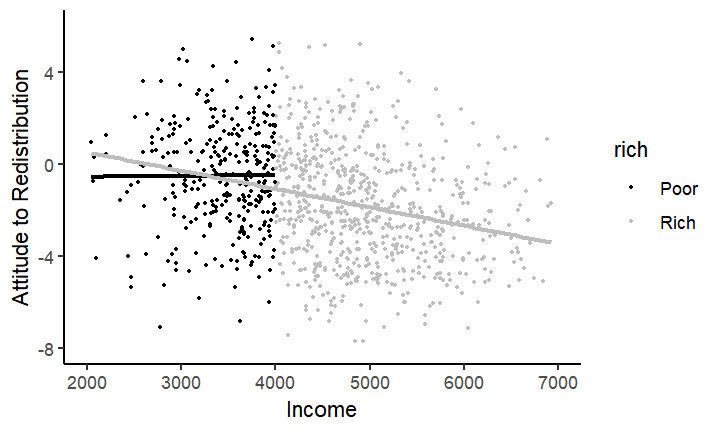
\includegraphics[width=\maxwidth]{figure/selection2-1} 

\end{knitrout}
\end{frame}

\begin{frame}
\frametitle{Selection Bias}
\begin{itemize}
\item There are four selection risks:
\begin{enumerate}
\item \textbf{Selection into existence:}
\begin{itemize}
\item Where do units (eg. political parties) come from?
\item Probably only parties that have a chance of success are formed
\item Does forming a party cause electoral success? Not for most people!
\end{itemize}
\end{enumerate}
\end{itemize}
\end{frame}

\begin{frame}
\frametitle{Selection Bias}
\begin{itemize}
\item There are four selection risks:
\begin{enumerate}
\setcounter{enumi}{1}
\item \textbf{Selection into survival:}
\begin{itemize}
\item Certain types of units disappear, so the units we see don't tell the full story
\end{itemize}
\end{enumerate}
\end{itemize}
\begin{multicols}{2}
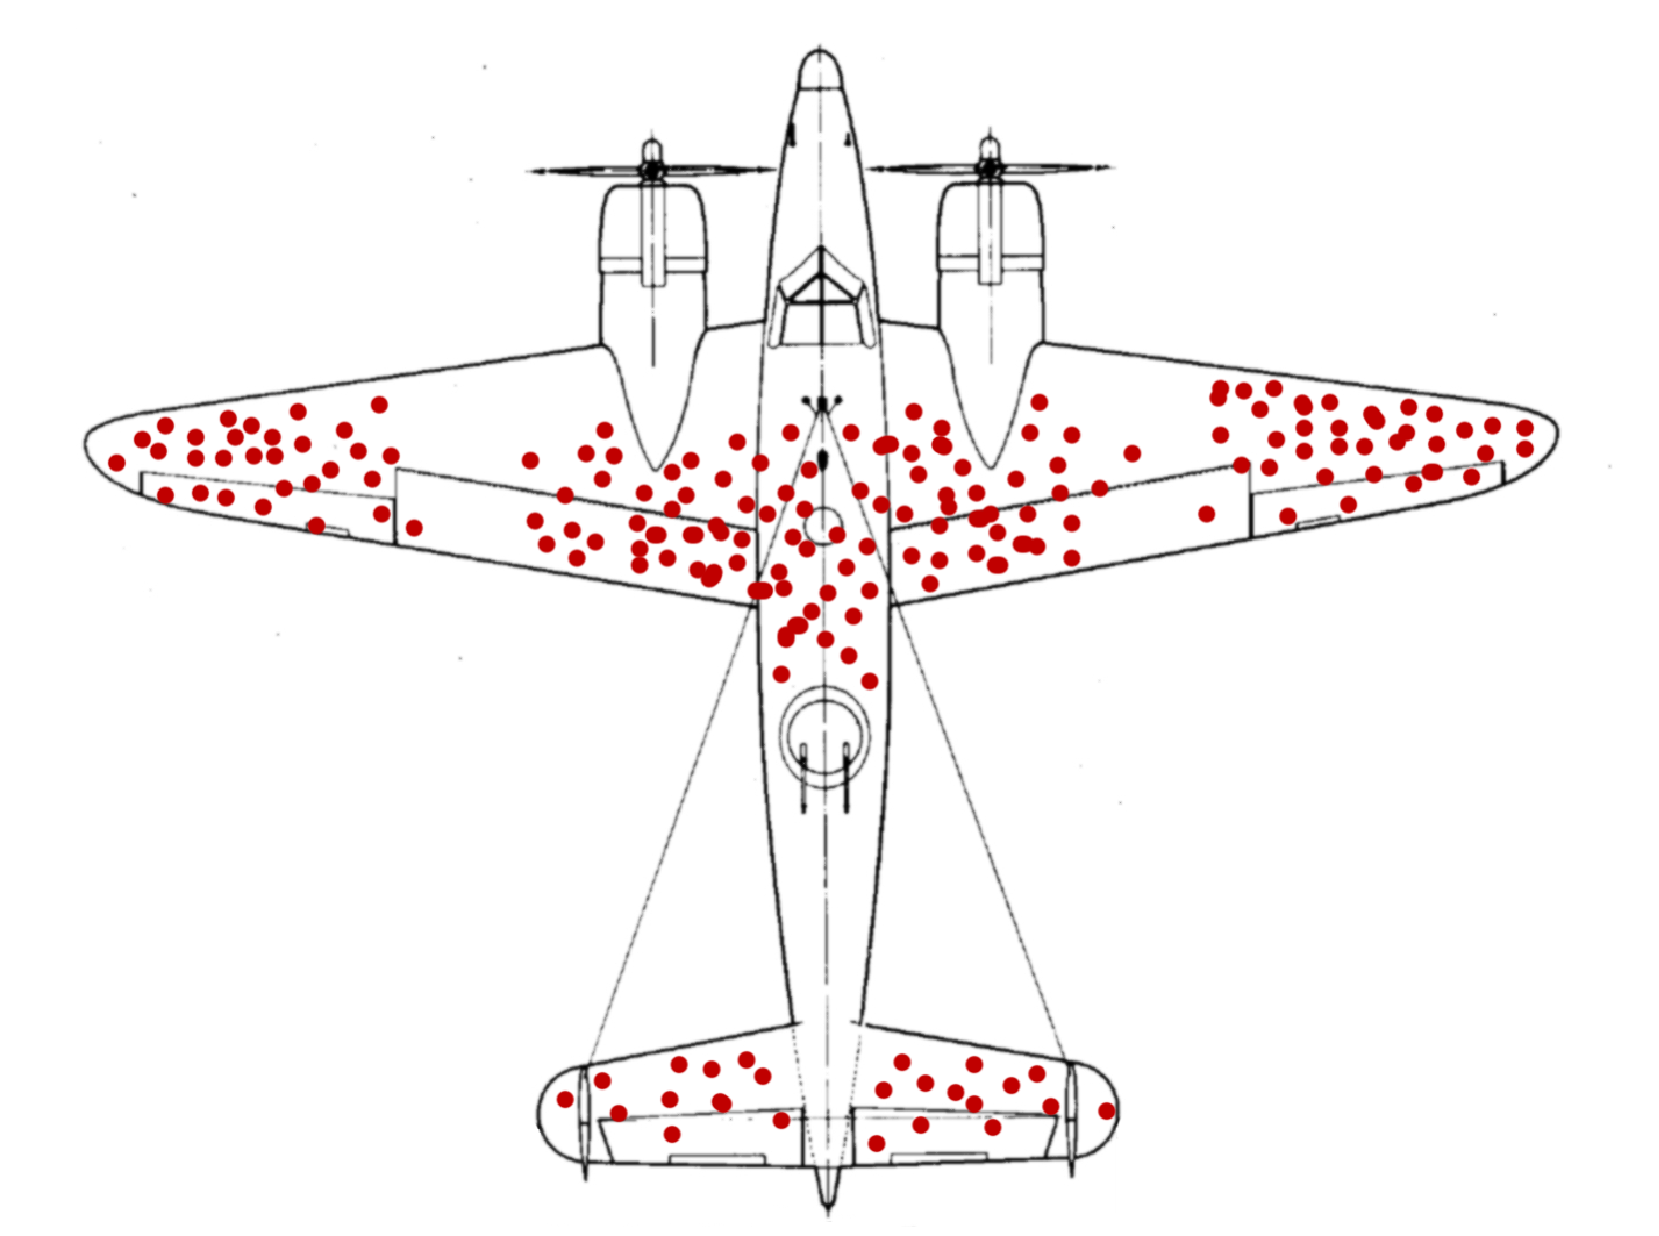
\includegraphics[scale=0.25]{Bombers.pdf}
\columnbreak
\begin{itemize}
\item Where would additional armour protect bombers?
\item Returned bombers got hit
\item But we do not know where \textit{bombers that did not return} got hit
\end{itemize}
\end{multicols}
\end{frame}

\begin{frame}
\frametitle{Selection Bias}
\begin{itemize}
\item There are four selection risks:
\begin{enumerate}
\setcounter{enumi}{2}
\item \textbf{Selection into the dataset:}
\begin{itemize}
\item Our dataset may not be representative
\item Only units with particular values of $X$ and $Y$ enter the dataset
\item Eg. If survey respondents who refuse are different from those who respond
\end{itemize}
\end{enumerate}
\end{itemize}
\end{frame}

\begin{frame}
\frametitle{Selection Bias}
\begin{itemize}
\item There are four selection risks:
\begin{enumerate}
\setcounter{enumi}{3}
\item \textbf{Selection into treatment:}
\begin{itemize}
\item All units are in our dataset, but they \textit{choose} their treatment value
\item Who chooses treatment? Those with the most to benefit, i.e. depending on $Y$!
\item Applying treatment to the others would probably have a very different effect
\end{itemize}
\end{enumerate}
\end{itemize}
\end{frame}

\begin{frame}
\frametitle{Measurement Bias}
\begin{itemize}
\item What happens if we measure our variables wrongly?
\footnotesize
\begin{table}[htbp]
  \centering
  \caption{Effects of Measurement Error}
    \begin{tabular}{|l|l|p{4cm}|}
    \hline
          & Measured with Bias & Measured with Random Noise \bigstrut\\
    \hline
    Outcome Variable & Effect biased & No bias but wider standard errors \bigstrut\\
    \hline
    Treatment Variable & Effect biased & Effect biased to zero \bigstrut\\
    \hline
    \end{tabular}%
  \label{tab:addlabel}%
\end{table}%
\normalsize
\end{itemize}
\end{frame}

\begin{frame}
\frametitle{Measurement Bias}
\begin{itemize}
\item What happens if we measure our variables wrongly?
\item No extra noise:
\end{itemize}
\begin{multicols}{2}
\begin{knitrout}
\definecolor{shadecolor}{rgb}{0.969, 0.969, 0.969}\color{fgcolor}
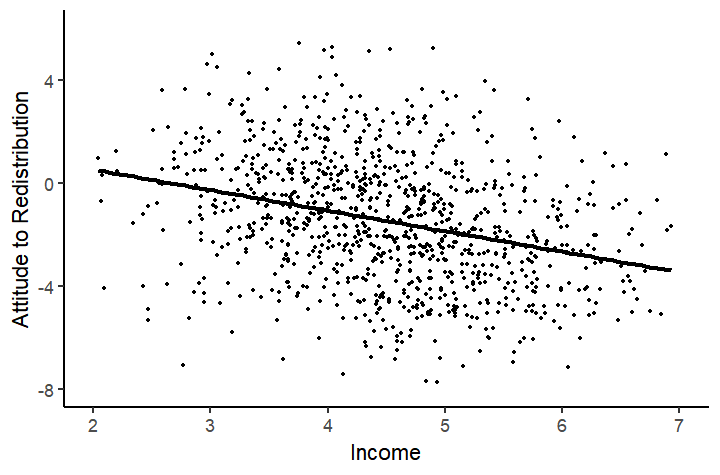
\includegraphics[width=\maxwidth]{figure/measure2-1} 

\end{knitrout}
\columnbreak

\begin{table}[!htbp] \centering 
  \caption{} 
  \label{} 
\tiny 
\begin{tabular}{@{\extracolsep{1pt}}lc} 
\\[-1.8ex]\hline 
\hline \\[-1.8ex] 
 & \multicolumn{1}{c}{\textit{Dependent variable:}} \\ 
\cline{2-2} 
\\[-1.8ex] & redist \\ 
\hline \\[-1.8ex] 
 income & $-$0.818$^{***}$ (0.078) \\ 
  Constant & 2.235$^{***}$ (0.361) \\ 
 \hline \\[-1.8ex] 
Observations & 1,000 \\ 
\hline 
\hline \\[-1.8ex] 
\textit{Note:}  & \multicolumn{1}{r}{$^{*}$p$<$0.1; $^{**}$p$<$0.05; $^{***}$p$<$0.01} \\ 
\end{tabular} 
\end{table} 

\end{multicols}
\end{frame}

\begin{frame}
\frametitle{Measurement Bias}
\begin{itemize}
\item What happens if we measure our variables wrongly?
\item Noise in the \textbf{outcome variable}:
\end{itemize}
\begin{multicols}{2}
\begin{knitrout}
\definecolor{shadecolor}{rgb}{0.969, 0.969, 0.969}\color{fgcolor}
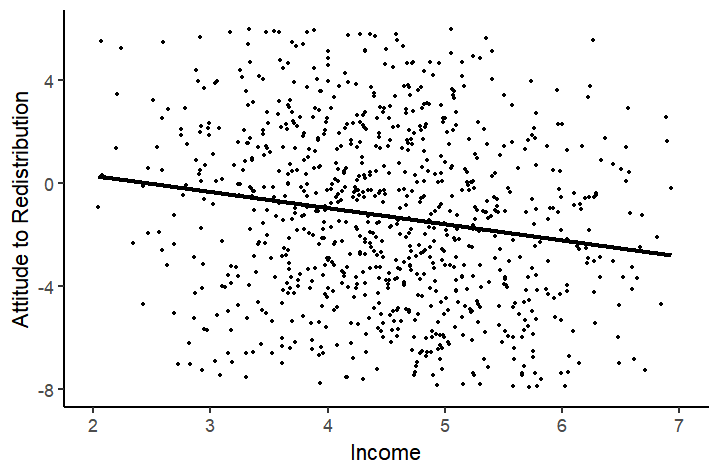
\includegraphics[width=\maxwidth]{figure/measure2b-1} 

\end{knitrout}
\columnbreak

\begin{table}[!htbp] \centering 
  \caption{} 
  \label{} 
\tiny 
\begin{tabular}{@{\extracolsep{1pt}}lc} 
\\[-1.8ex]\hline 
\hline \\[-1.8ex] 
 & \multicolumn{1}{c}{\textit{Dependent variable:}} \\ 
\cline{2-2} 
\\[-1.8ex] & redist \\ 
\hline \\[-1.8ex] 
 income & $-$0.790$^{***}$ (0.138) \\ 
  Constant & 1.956$^{***}$ (0.637) \\ 
 \hline \\[-1.8ex] 
Observations & 1,000 \\ 
\hline 
\hline \\[-1.8ex] 
\textit{Note:}  & \multicolumn{1}{r}{$^{*}$p$<$0.1; $^{**}$p$<$0.05; $^{***}$p$<$0.01} \\ 
\end{tabular} 
\end{table} 

\end{multicols}
\end{frame}

\begin{frame}
\frametitle{Measurement Bias}
\begin{itemize}
\item What happens if we measure our variables wrongly?
\item Noise in the \textbf{explanatory} variable:
\end{itemize}
\begin{multicols}{2}
\begin{knitrout}
\definecolor{shadecolor}{rgb}{0.969, 0.969, 0.969}\color{fgcolor}
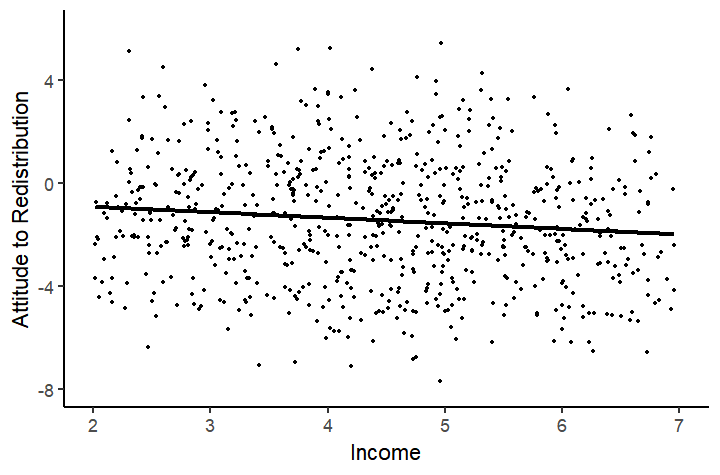
\includegraphics[width=\maxwidth]{figure/measure2c-1} 

\end{knitrout}
\columnbreak

\begin{table}[!htbp] \centering 
  \caption{} 
  \label{} 
\tiny 
\begin{tabular}{@{\extracolsep{1pt}}lc} 
\\[-1.8ex]\hline 
\hline \\[-1.8ex] 
 & \multicolumn{1}{c}{\textit{Dependent variable:}} \\ 
\cline{2-2} 
\\[-1.8ex] & redist \\ 
\hline \\[-1.8ex] 
 income & $-$0.187$^{***}$ (0.037) \\ 
  Constant & $-$0.620$^{***}$ (0.183) \\ 
 \hline \\[-1.8ex] 
Observations & 1,000 \\ 
\hline 
\hline \\[-1.8ex] 
\textit{Note:}  & \multicolumn{1}{r}{$^{*}$p$<$0.1; $^{**}$p$<$0.05; $^{***}$p$<$0.01} \\ 
\end{tabular} 
\end{table} 

\end{multicols}
\end{frame}

\begin{frame}
\frametitle{Lack of Overlap}
\begin{itemize}
\item Regression normally helps us pick appropriate comparisons
\begin{itemize}
\item Eg. Comparing only among men, what is the effect of income on attitudes to redistribution? 
\end{itemize}
\item But what if there are no women with high income?
\item Regression \textit{creates} comparisons for us
\begin{itemize}
\item How? That's where the functional for of the regression comes in
\item A linear regression interpolates/extrapolates \textit{linearly} to 'create' comparison cases
\end{itemize}
\item Lack of overlap probably means we \textit{cannot} explain outcomes with this data
\end{itemize}
\end{frame}

\begin{frame}
\frametitle{Lack of Overlap}
\begin{knitrout}
\definecolor{shadecolor}{rgb}{0.969, 0.969, 0.969}\color{fgcolor}
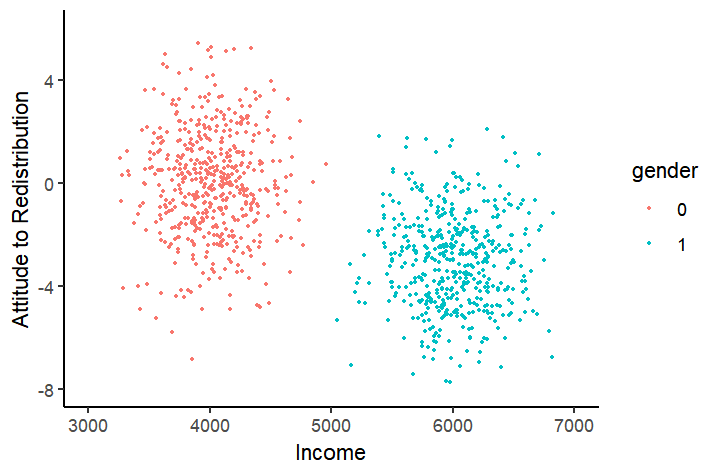
\includegraphics[width=\maxwidth]{figure/overlap1-1} 

\end{knitrout}
\end{frame}

\begin{frame}
\frametitle{Lack of Overlap}
\begin{knitrout}
\definecolor{shadecolor}{rgb}{0.969, 0.969, 0.969}\color{fgcolor}
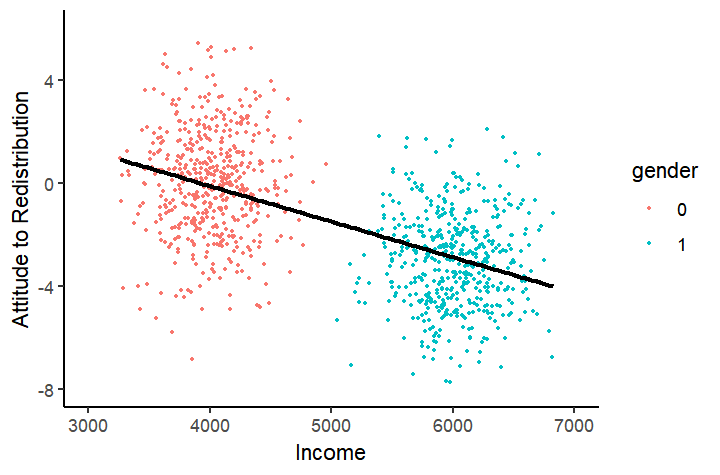
\includegraphics[width=\maxwidth]{figure/overlap2-1} 

\end{knitrout}
\end{frame}

\begin{frame}
\frametitle{Lack of Overlap}
\begin{knitrout}
\definecolor{shadecolor}{rgb}{0.969, 0.969, 0.969}\color{fgcolor}
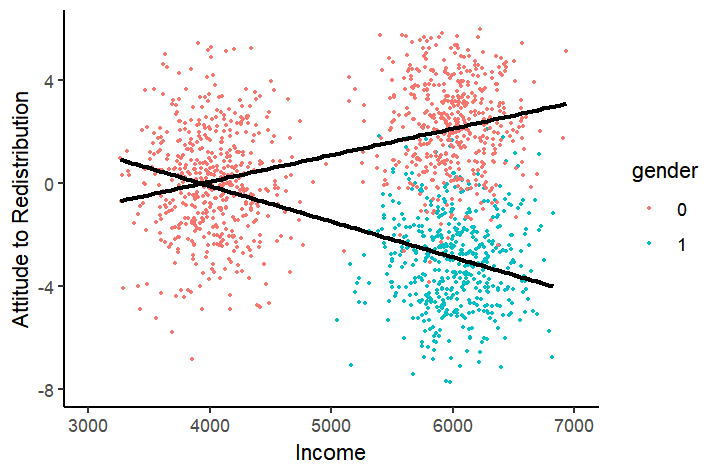
\includegraphics[width=\maxwidth]{figure/overlap3-1} 

\end{knitrout}
\end{frame}

\begin{frame}
\frametitle{Lack of Overlap}
\begin{itemize}
\item With more than a few variables, lack of overlap is \textit{guaranteed}
\item 6 variables with 10 categories each = $10^6 = 1,000,000$ possibilities, and a sample of maybe 5,000?
\item Common datasets have 0\% counterfactuals present in the data (King 2006)
\begin{itemize}
\item How many 45 year-old female accountants with a PhD and a cat who live in Centro are there?
\item And we need some that are low-income and some that are high-income
\end{itemize}
\item A problem of \textbf{multi-dimensionality}
\item And of \textbf{model dependence} - our results depend on the functional form in our regression model
\end{itemize}
\end{frame}




% Overlap/Functional form error
% Measurement Error
% Omitted Variable Bias
% Reverse Causation/Endogeneity
% Self-Selection Bias
% Data Selection Bias

% Stress - in prep for week 2 - that regression only buys you (conditional) correlation

%Chenage all examples to age-gender-income

\end{document}


%setwd('C:\\Users\\Jonny\\Google Drive\\Academic\\USP\\Class\\Week 1 - Intro\\Lecture Slides')
%knitr::knit("Slides_Wk1_intro_5.Rnw")
